\documentclass[%
master,    % тип документа
natbib,      % использовать пакет natbib для "сжатия" цитирований
subf,        % использовать пакет subcaption для вложенной нумерации рисунков
href,        % использовать пакет hyperref для создания гиперссылок
colorlinks,  % цветные гиперссылки
%fixint,     % включить прямые знаки интегралов
]{disser}

\usepackage[
a4paper, mag=1000,
left=2.5cm, right=1cm, top=2cm, bottom=2cm, headsep=0.7cm, footskip=1cm
]{geometry}

\usepackage[intlimits]{amsmath}
\usepackage{amssymb,amsfonts}

\usepackage[T2A]{fontenc}
\usepackage[utf8]{inputenc}
\usepackage[english,russian]{babel}
\ifpdf\usepackage{epstopdf}\fi
\usepackage[autostyle]{csquotes}

% Шрифт Times в тексте как основной
%\usepackage{tempora}
\usepackage{setspace}
\usepackage{mathtools}
% альтернативный пакет из дистрибутива TeX Live
%\usepackage{cyrtimes}
\usepackage{listings}
% Шрифт Times в формулах как основной
%\usepackage[varg,cmbraces,cmintegrals]{newtxmath}
% альтернативный пакет
%\usepackage[subscriptcorrection,nofontinfo]{mtpro2}

% Плавающие рисунки "в оборку".
\usepackage{wrapfig}

% Номера страниц снизу и по центру
%\pagestyle{footcenter}
%\chapterpagestyle{footcenter}

% Точка с запятой в качестве разделителя между номерами цитирований
%\setcitestyle{semicolon}

% Использовать полужирное начертание для векторов
\let\vec=\mathbf
%______________________________-
\usepackage{lipsum}

%\usepackage{titlesec}
%\usepackage{spacing}
%\titleformat{\section}[block]{\color{blue}\Large\bfseries\filcenter}{}{1em}{}
% Номера страниц снизу и по центру
\pagestyle{footcenter}
\chapterpagestyle{footcenter}

% Точка с запятой в качестве разделителя между номерами цитирований
%\setcitestyle{semicolon}



% Переопределение стандартных заголовков
%\def\contentsname{Содержание}
%\def\conclusionname{Выводы}
%\def\bibname{Литература}

\usepackage{geometry} % пакет для установки полей
\geometry{top=1.5cm} % отступ сверху
\geometry{bottom=2cm} % отступ снизу
\geometry{left=3cm} % отступ справа
\geometry{right=1.5cm} % отступ слева
\newcommand{\sectionbreak}{\clearpage}
\newcommand*{\No}{\textnumero}
\renewcommand{\Re}{\mathrm{Re}}
\renewcommand{\Im}{\mathrm{Im}}

\newcommand{\const}{\mathrm{const}}
\newcommand{\arccosh}{\mathrm{arccosh}}

\newcommand{\vF}{\mathbf{F}}
\newcommand{\ve}{\mathbf{e}}
\newcommand{\vk}{\mathbf{k}}
\newcommand{\vq}{\mathbf{q}}
\newcommand{\vp}{\mathbf{p}}
\newcommand{\va}{\mathbf{a}}
\newcommand{\vP}{\mathbf{P}}
\newcommand{\vK}{\mathbf{K}}
\newcommand{\vQ}{\mathbf{Q}}
\newcommand{\vA}{\mathbf{A}}
\newcommand{\vr}{\mathbf{r}}
\newcommand{\vR}{\mathbf{R}}

\newcommand{\vRR}{\boldsymbol{\mathcal{R}}}
\newcommand{\veps}{\boldsymbol{\varepsilon}}

\newcommand{\cA}{\mathcal{A}}
\newcommand{\cR}{\mathcal{R}}
\newcommand{\cM}{\mathcal{M}}
\newcommand{\cE}{\mathcal{E}}
\newcommand{\cJ}{\mathcal{J}}
\newcommand{\cT}{\mathcal{T}}
\newcommand{\cD}{\mathcal{D}}


%______________________________-
% Включать подсекции в оглавление
\setcounter{tocdepth}{2}

\graphicspath{{fig/}}

\begin{document}
\title{Моделирование нуклеосинтеза в звездах}
\maketitle
\section*{\centering Введение}
\addcontentsline{toc}{section}{Введение}
Вопрос о том, из чего состоит материальный мир стоит перед учеными с самого зарождения науки Левкипп (около 430 г. до н.э.) и Демокрит (около 420 г. до н.э.) первыми предложили атомную теорию, в которой вся материя состоит из неделимых частиц. Позже ученые добились успехов в экспериментах с процессами возникновения различных веществ. Алхимики, например, задавались вопросами преобразования обычных металлов (свинца, например) в благородные (такие как золото). Попытки их были тщетны, и теоретическая основа этих преобразований не получила никакого развития. И только в конце XX века ядерные физики добились успеха превращения висмута в золото (лишь в небольших количествах и с коммерческими расходами)
В связи с развитием ядерной физики были также построено огромное количество различных математических моделей, объясняющих возникновение тяжелых элементов, а именно тяжелее железа, из более легких.

В данной работе, будут моделироваться такие реакции с использование открытой библиотеки реакций ReacLib, в основе которой лежит построение сечения зависимостью от температуры по 7 параметрам. Данная библиотека уже включает в себя некоторый набор реакций, приводящий к появлению обойденных ядер, но нас интересуют только реакции, в которых участвует столкновительный $\beta$-распад

Основной целью работы является построение сечений для столкновительного $\beta$-распада для столкновении элементов с протоном, а также оценка влияния этих реакций на полученную распространенность элементов в результате всех процессов за промежуток времени.

Сам процесс моделирования будет выполняться с помощью открытой библиотеки SkyNet, написанную Jonas Lippuner с дополнение ее своим набором реакций.

\section{Столкновительный $\beta$-распад}
Данный процесс является одним из процессов, приводящих к появлению обойденных ядер.

Обойдённые ядра - устойчивые атомные ядра, лежащие в стороне от всех возможных путей образования тяжёлых ядер из более лёгких в процессе последовательного захвата последними нейтронов \cite{reactions}. Распространённость обойденных ядер, как правило, примерно на два порядка величины ниже, чем у близких к ним ядер, лежащих на пути нейтронного захвата. К таковым относятся: $^{74}Se$, $^{78}Kr$, $^{80}Kr$, $^{84}Sr$, $^{92}Mo$, $^{94}Мо$, $^{96}Ru$, $^{98}Ru$, $^{102}Pd$, $^{106}Cd$, $^{108}Cd$, $^{113}In$, $^{112}Sn$, $^{114}Sn$, $^{115}Sn$, $^{120}Te$, $^{124}Xe$, $^{126}Xe$, $^{130}Ba$, $^{132}Ba$, $^{136}Ce$, $^{138}Ce$, $^{144}Sm$, $^{152}Gd$, $^{152}Dy$, $^{158}Dy$, $^{162}Er$, $^{164}Er$, $^{168}Yb$, $^{174}Hf$, $^{180}W$, $^{184}Os$, $^{190}Pt$, $^{196}Hg$ \cite{role}.

Столкновительный $\beta-$распад стабильных ядер, инициируемый их кулоновскими столкновениями с другими ядерными частицами звездной среды, может быть основой модели процесса синтеза обойденных ядер.
Проблема их синтеза на основе физического механизма захвата нейтронов ($s-$ или $r-$процесса) состоит в прерывании цепочки последовательных $\beta-$распадов на $\beta$-стабильном ядре $(A,Z)$.

Процесс СБР стабильных ядер, о котором говорилось выше, для нуклидов главной последовательности предоставляет еще одну возможность преодолеть энергетический порог и осуществить переход 
$$(A,Z) \xrightarrow[]{\beta^-} (A,Z + 1)$$
, открывая путь к последующему естественному $\beta$-переходу
$$(A,Z+1) \xrightarrow[]{\beta^-} (A,Z + 2)$$

Может оказаться, что при этом малость сечений для процесса такого рода уже не будет играть особой роли, если будут не малы плотность вещества в недрах звезды и временная протяженность квазиравновесной стадии звездной эволюции.

Расчеты показывают, что модель синтеза обойденных элементов в звездном веществе на этапе квазиравновесной стадии, основанная на явлении СБР стабильных ядер главной последовательности, качественно, а в ряде случаев и количественно, способна воспроизвести нерегулярный ход кривой относительной распространенности обойденных ядер. Этот факт можно расценивать как косвенное свидетельство в пользу реальности явления столкновительного $\beta$-распада стабильных ядер \cite{tak}.

В случае столкновительного $\beta$-распада возможно несколько видов процессов, а именно: протон-ядерные, ядро-ядерные и процесс, стимулированный нейтронами. Рассчитанные сечения для протон-ядерных и ядро-ядерных оказались невелики (менее $10^{-50}cm^2$), и процесс пока не доступен для прямого наблюдения, но при помощи программного обеспечения, позволяющего моделировать данные процессы мы можем оценить влияние их на конечные распространенности элементов \cite{tak_article}. Наряду с кулоновскими столкновениями ядер можно предложить механизм СБР, не связанный с кулоновскими силами и в то же время незамаскированный возможным появлением продуктов $\beta$-распада за счет ядерных реакций. Речь идет о процессе СБР ядра, стимулированном столкновениями с нейтронами.

Данная работа рассматривает в первую очередь влияние протон-ядерного столкновения на процессы, протекающие в нейтронных звездах, а именно r-process, так как концентрация протонов при этом достаточно велика, чтобы это влияние оказалось существенным. 

Сечение для столкновительного $\beta$ распада получим через формулу (\ref{eq:sigma}).

\begin{equation}
\label{eq:sigma}
\begin{split}
\sigma_\beta^{(col)}(\beta_f) =
\frac{4\sqrt{2}}{\pi}\frac{g_v^2\alpha_e^4 Z (Z + 1)Z'^4\mu^{9/2}}{\epsilon_i^{3/2}(1-\exp(-2\pi\lambda_i))}\xi_\beta(\beta_f) \times \\
\int_{0}^{\xi_i-\Delta-\Delta_f}\frac{\Phi(E_f)d\epsilon_f}{(\exp(2\pi\lambda_f)-1)k_f(k_i-k_f)^4(k_i+k_f)^2} \times \\
\int_{x_0}^{0}\frac{\left|F(-i\lambda_i,-i\lambda_f,1;x)\right|^2}{(1-x)^2}dx,
\end{split}
\end{equation}

где $E_f = \epsilon_i - \epsilon_f - \Delta - \Delta_f$, $x_0 = -4 k_i k_f / (k_i - k_f)^2$, а функция $\Phi(E)$ имеет вид:

$$
\Phi(E) = \frac{1}{60}(E^2-1)^{1/2}(2E^4-9E^2-8)+\frac{1}{4}E\ln(E+(E^2-1)^{1/2})
$$


(!!!)Место для второй формулы

Для возможности использования полученных сечений вместе с другими библиотеками ядерных реакций необходимо привести их к единому формату. Данным форматом был выбран REACLIB.

\section{REACLIB}

База данных JINA REACLIB полностью открыта и доступна для сообщества через интернет. Текущая версия библиотеки хранит показатели реакций, таких как зависимость от температуры через семи-параметрическое приближение \cite{jina}.

$$\lambda = \exp \bigg[a_0 + \sum_{i=1}^{5}a_iT_9^{\frac{2i-5}{3}}+a_6 \ln T_9\bigg]$$

Чтобы получить параметры $a_0, .., a_6$ для каждой из наших реакций мы воспользуемся статистической моделью.

Модель представляет из себя усредненные коэффициенты перехода T. Они не отражают резонансное поведение, но описывают эффект поглощения чере мнимую часть в (оптическом) ядро-ядро потенциале, что приводит к известному выражению:


\begin{multline}
\sigma^{\mu\nu} = \\
= \frac{\pi\hbar/(2\mu_{ij}E_{ij})}{(2J_i^\mu+1)(2J_j+1)}\sum_{J,\pi}(2J + 1) \\
\times \frac{T_j^\mu(E,J,\pi,E_i^mu, J_i^\mu,\pi_i^\mu)T_0^\nu(E,J,\pi,E_m^\mu,J_m^\nu,\pi_m^\nu)}{T_{tot}(E,J,\pi)}
\end{multline}

для сечения $\sigma^{\mu\nu}$ реакции $i^\mu(j,o)m^\mu$ из состояния $i^\mu$ в состояние $m^\nu$ конечного ядра с центром энергии масс $E_{ij}$ и уменьшенной массой $\mu_ij$.

Показатели реакций были посчитаны для набора из 24 температур: $T_9$ = 0.1,0.15, 0.2, 0.3, 0.4, 0.5, 0.6, 0.7, 0.8, 0.9, 1.0, 1.5, 2.0, 2.5, 3.0, 3.5, 4.0, 4.5, 5.0, 6.0, 7.0, 8.0, 9.0, 10.0. Для простого применения в астрофизических исследованиях все виды реакций ($(n,\gamma)$, $(n,p)$, $(p,\alpha)$, $(p, \gamma)$, (p, n), $(p, \alpha)$, $(\alpha, \gamma)$, $(\alpha, n)$, $(\alpha, p)$, $(\gamma, n)$, $(\gamma, p)$, $(\gamma, \alpha))$ аппроксимируются через единое приближение вида

\begin{equation}
\label{eq:system}
\begin{split}
\left.
	\begin{array}{ccc}
		N_{A}\langle \sigma v \rangle \\
		\lambda_\gamma
	\end{array}
\right\}
 = \exp (a_0 + a_1 T_9^{-1} + a_2 T_9^{-1/3} + \\
a_3 T_9^{1/3} + a_4 T_9 + a_5 T_9^{5/3} + a_6 \ln T_9)
\end{split}
\end{equation}

c 7 открытыми параметрами $a_0$ - $a_6$, где $T_9$ это $10^9$К.

Данное приближение является достаточно гибким чтобы удовлетворить различным температурным зависимостям для различных видов реакций в промежутке температур $0.001 \le T_9 \le 10$ \cite{rates}.

\section{SkyNet}

Программный пакет SkyNet представляет из себя обще-целевую сеть ядерных реакций, специально разработанную для моделирования r-процесса, но она также применима к другим астрофизическим сценариям \cite{skynet}.

SkyNet написан на языке C++ и имеет модульную архитектуру. Помимо сети ядерных реакций, он также включает в себя модуль решения ядерного статистического равновесия (!!! Nuclear Statistical equilibrium), уравнение состояния Гельмгольца. SkyNet также моделирует эволюцию температуры, отслеживая изменение энтропии при ядерных реакциях и распадах.

SkyNet также имеет обертку для использования ее с Python, что делает очень удобным использование его через интерактивные оболочки.

Важно отметить, что SkyNet успешно прошел сравнения с другими аналогичным ПО (WinNet, XNet) и даже, приблизился к симуляции Seitenzahl \cite{simulation}.

(!!! мало информации, нужно найти больше)

\section{Расчеты}
Сначала были получены сечения столкновительного бета-распадов при столкновении ядра с протоном, такие как, например:
$$^{130}Xe \to ^{130}Cs$$
Для этого была написана программа, в результате работы которой, был построен график (рис. \ref{ris:1}).
\begin{figure}[h]
	\center{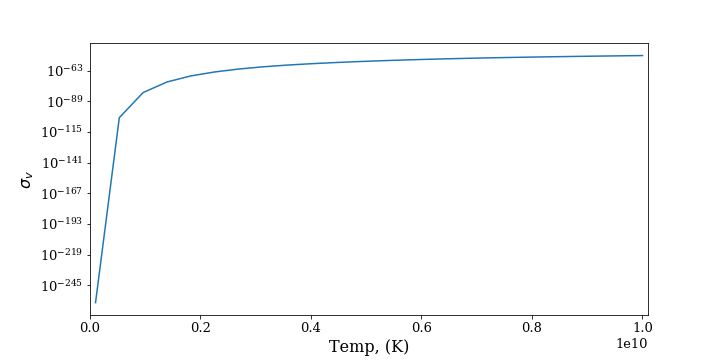
\includegraphics[width=0.8\linewidth]{xe130-cs130}}
	\caption{Сечение для СБР при столкновении $^{130}Cs$ с протоном}
	\label{ris:1}
\end{figure}
Полученные 24 значения температур являются избыточными в нашем случае, так целью является параметризация данной зависимости через 7 параметров $a_0, ..., a_6$ (\ref{eq:system}). То есть мы имеет 17 лишних уравнений. Поэтому для решения переопределенной системы воспользуемся методом наименьших квадратов (\ref{ris:2}).

\begin{figure}[h]
	\center{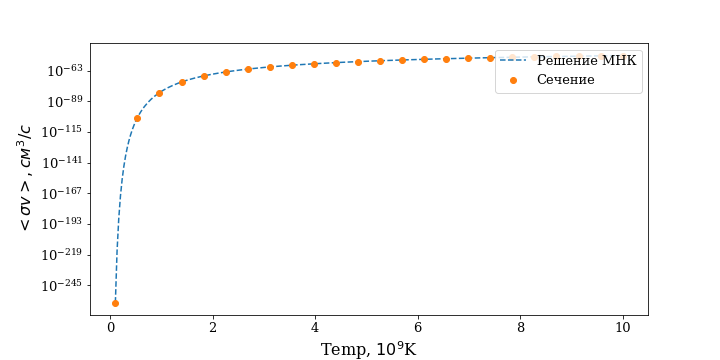
\includegraphics[width=0.8\linewidth]{compare-xe130-cs130}}
	\caption{Сравнение решения методов наименьших квадратов с полученным сечением}
	\label{ris:2}
\end{figure}

Далее, составим необходимый для REACLIB файл библиотеки реакций. Для перехода $^{130}Xe \to ^{130}Cs$ получаем строки вида: 

\begin{lstlisting}[label={lst:label}]
	5
	         pxe130cs130    p                  cleaw     0.00000e+00          
	 3.631089e+01-2.513083e+01-3.379005e+02 1.434772e+02                      
	-2.028014e+00-6.306473e-02-1.208779e+02                                   
	
\end{lstlisting}

В данном файле стоит отметить факт явного указания $p$ - протона в качестве участника реакции, так как сечение СБР зависит от концентрации протонов. Также важно указать флаг "w", указывающий, что реакция является "слабой" и SkyNet толерантно относился к нарушению закона сохранения заряда (данный программный пакет не позволяет учесть потерю электрона (!!!)).

Построим также графическое представление параметров $a$ для некоторых реакций (!!! смотри другую сторону) (рис. \ref{ris:result-a}).

\begin{figure}[h]
	\center{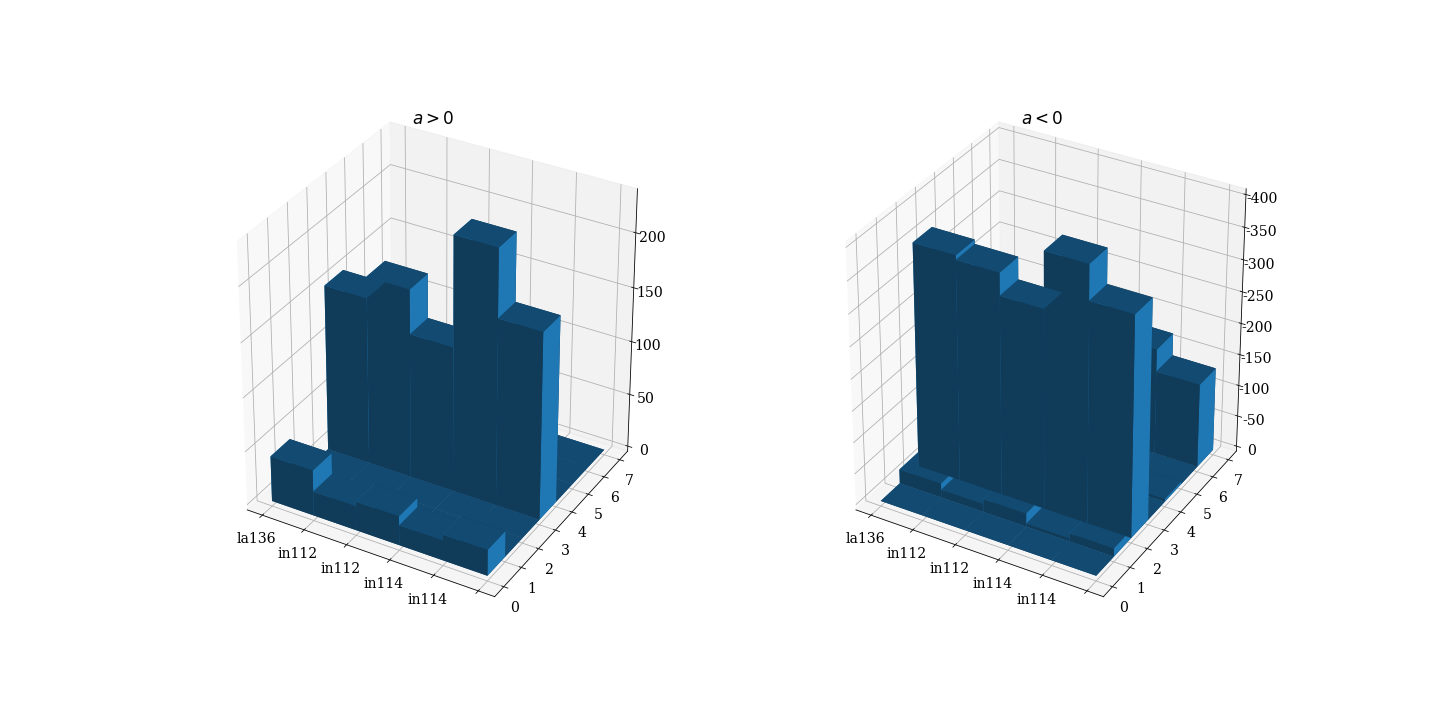
\includegraphics[width=0.7\linewidth]{result-a}}
	\caption{Конечные распространенности обойденных ядер}
	\label{ris:result-a}
\end{figure}

Для моделирования ядерных реакций воспользуемся включенной в SkyNet моделю r-process. Она содержит список из 7836 ядер, участвующих в реакциях, начальные распространенности этих ядер, а также зависимости плотности и температуры от времени. Эволюция протекает в промежутке времени от $1.21\times 10^{-3}c$ до $5\times 10^8c$. 

Изначально, если оставлять файл JINA REACLIB в таком виде, в котором он присутствует в библиотеке, влияние добавленных мною реакций отсутствовало. Это связано с тем, что в сети уже присутствовали реакции с этими элементами, но гораздо большим сечением, которое перекрывает наши реакции. Добится хоть какого-то влияния на небольших температурах невозможно, так как по характеру графика на рисунке (\ref{ris:1}) можно заметить его быстрое затухание при стремлении температуры справа к $10^8 K$, а именно при относительно низких ($10^9 K$) температурах протекает большая часть эволюции.

Чтобы увидеть влияние СБР, сначала мы пошли по пути удаления из файла нашей библиотеки реакций протона (чтобы SkyNet игнорировал концентрацию протонов), а также явного указания количества протонов (как множитель перед $\sigma_v$). Полученная разница между распространенностями оказалась незначительна даже при больших концентрациях протонов (!!! сколько 1e40?), поэтому мы пришли к выводу что для оценки возникновения обойденных ядер через СБР процесса можно изменить REACLIB таким образом, чтобы только столкновительный $\beta$-распад производил обойденные ядра, остальные же процессы на данном этапе отбросим.

Из REACLIB были удалены реакции вида (\ref{eq:remove1}), а именно те, которые приводят к образованию обойденного ядра, но при этом не являются $\beta$-распадом. Было исключено 168 реакций.

\begin{equation}
\label{eq:remove1}
	^{79}Br \to ^{78}Br + n
\end{equation}

Полученные данные представляют из себя иерархический формат данных h5. Извлекая конечные распространенности, видим результат для всех обойденных ядер (рис. \ref{ris:result}):

\begin{figure}[h]
	\center{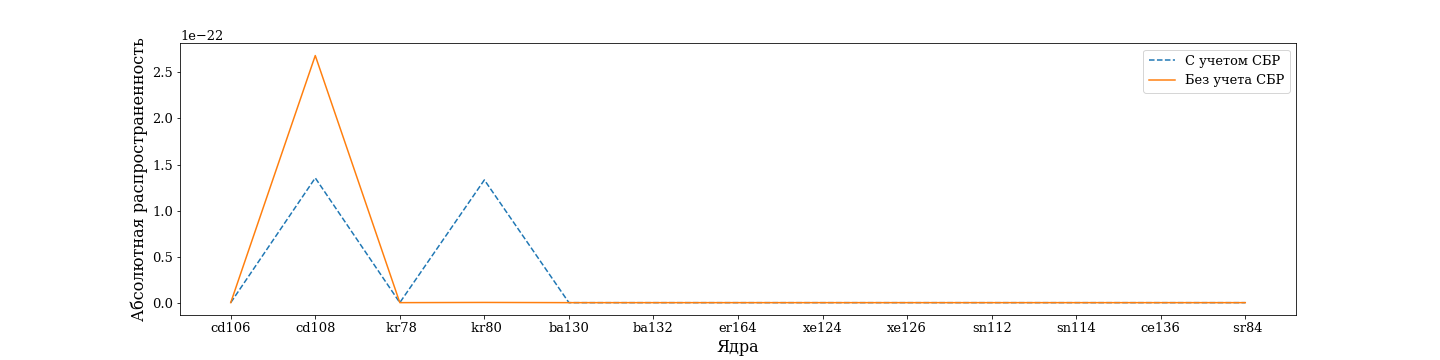
\includegraphics[width=1\linewidth]{result}}
	\caption{Конечные распространенности обойденных ядер}
	\label{ris:result}
\end{figure}

Построим график относительной ошибки между нашей библиотекой и тем, что уже присутствовало в REACLIB (рис. \ref{ris:result-err}):

\begin{figure}[h]
	\center{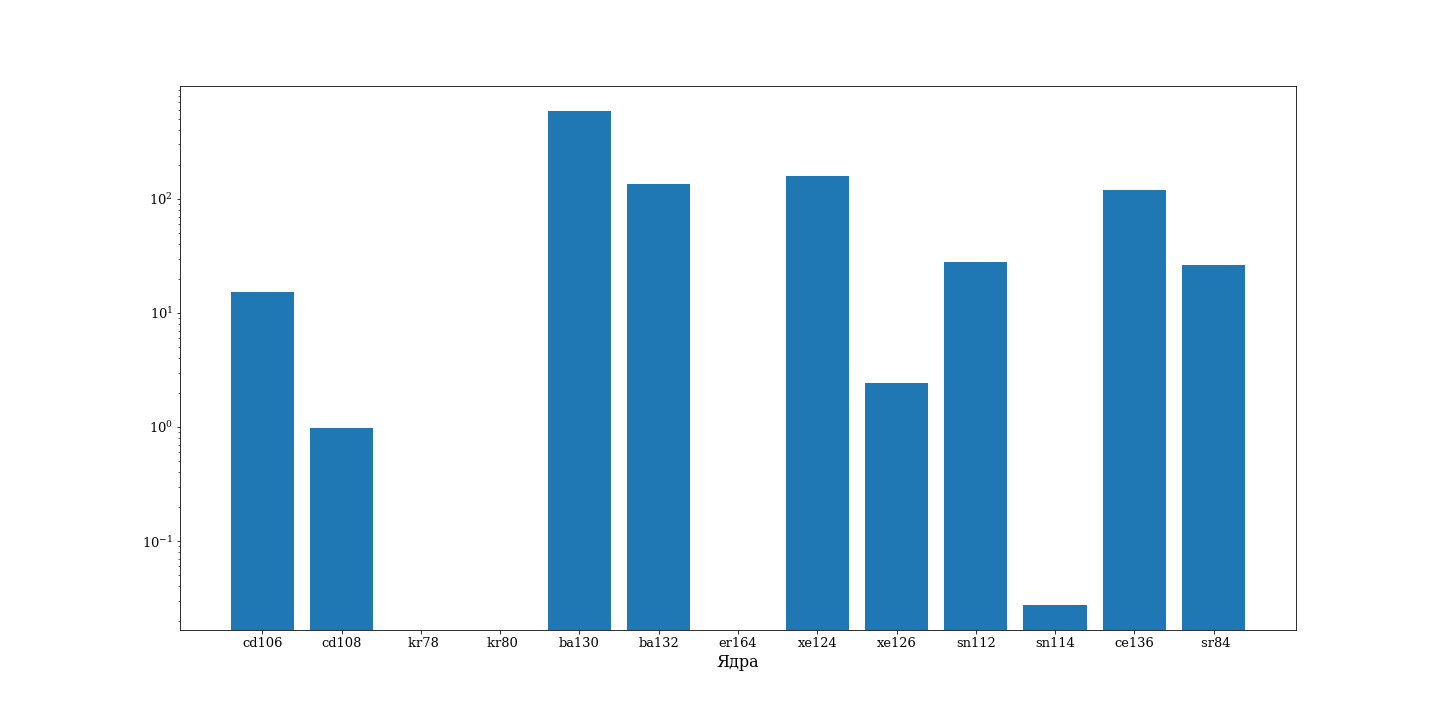
\includegraphics[width=1\linewidth]{result-err}}
	\caption{Относительная ошибка при сравнении стандартной библиотеки реакций SkyNet и библиотеки, включающей СБР}
	\label{ris:result-err}
\end{figure}

С учетом того, что мы полностью удалили все реакции, приводящие к возникновению обойденных $\beta$ ядер из сети реакций, полученная разница в их распространенностях оказалась не так велика, что говорит о том, что наши реакции действительно учитывались и смогли смоделировать возникновение некоторого количества обойденных ядер.

\section{Заключение}

В данной работе было рассмотрено влияние столкновительного бета распада на эволюцию звездных процессов. На языке Python был получено сечения для столкновительного процесса некоторых ядер с протоном. При помощи программного пакета SkyNet, а также дополнения библиотеки JINA REACLIB было подтверждено, что СБР может являться источником обойденных ядер и при больших значениях сечения это влияние существенно, но конкретно для ситуации столкновения с протоном, это влияние невелико даже для r-процесса. Чтобы увидеть эти изменения, пришлось удалить часть конкурирующих реакций, приводящих к образованию обойденных ядер, а именно, все, кроме $\beta$-распада.  

Данная работа рассматривает только часть образований материнских ядер, причем при столкновении с протоном. Также, для расширения списка реакций необходимо добавить столкновительные реакции для других ядер, а также нейтронов, сечения для которых намного выше, ввиду отсутствия Кулоновского барьера.

\bibliographystyle{utf8gost705u}
\bibliography{sample}
\end{document} 